\documentclass[10pt]{article}
\usepackage[margin=1in]{geometry}
\usepackage[T1]{fontenc}
\usepackage[utf8]{inputenc}
\usepackage{microtype}
\usepackage{amsmath,amssymb}
\usepackage{booktabs,tabularx,array,multirow}
\usepackage{graphicx}
\usepackage{xcolor}
\usepackage[numbers,sort&compress]{natbib}
\usepackage{hyperref}
\hypersetup{colorlinks=true,linkcolor=blue!50!black,citecolor=blue!50!black,urlcolor=blue!50!black}
\setlength{\parindent}{0pt}
\setlength{\parskip}{0.35em}
\renewcommand{\arraystretch}{1.12}
\newcolumntype{Y}{>{\raggedright\arraybackslash}X}
\newcolumntype{C}{>{\centering\arraybackslash}X}
\graphicspath{{./}{../figures/}}

\title{\textbf{Self-Correction Is Domain-Conditioned:}\\
\large Evidence for Different Knot Types in Math and Coding}
\author{Yuhan Chi\\Fudan University\\\texttt{masterwuguicyh@gmail.com}}
\date{}

\begin{document}
\maketitle

\begin{abstract}
Process supervision often assumes that self-correction in chain-of-thought (CoT) traces carries the same semantics across domains. This paper tests that assumption with a small interpretable probe used as a measurement tool rather than a new verifier. In noncoding domains, the signal is strong: on math, the probe reaches AUC-of-AUROC $0.958$ and AUROC@100\% $0.982$; on science, it reaches $0.799$ and $0.841$. Math also shows near-lossless frozen-basis transfer across anchors ($\Delta$AUROC $=-0.001$ forward), which points to an early reusable quality geometry. In coding, the same feature family fails: AUC-of-AUROC falls to $0.434$, below a $0.506$ token-confidence baseline, and the strongest full-scale lexical proxy, \texttt{condition\_reversal\_per1k}, has only $\rho=-0.062$. A one-hidden-layer MLP on the same 25 cached features preserves the same ordering, with mean anchor AUROC $0.941$ / $0.723$ / $0.497$ for math / science / coding.

The paper then adds a small study of \emph{local state breaks}. This part is not used to estimate prevalence or to claim a finished taxonomy. It asks a narrower question: does the same annotation logic transfer across domains, and do break-positive subsets preserve the same correctness geometry? The answer is asymmetric. Math explicit-state-break annotations remain coherent enough to support the usual geometry inside break-positive runs. Coding needs a separate execution-semantic protocol, and an expanded 240-run GLM-assisted audit still shows almost no relation between coding knot labels and correctness ($\rho=-0.023$ for knot severity; knot-present accuracy $0.537$ vs.\ $0.545$ when absent). A broader coding-side feature screen finds only modest alternatives, and the strongest static complexity feature does not support a monotone ``more complex $\rightarrow$ more wrong'' account. The paper therefore makes one main claim: CoT quality signals are strongly domain-conditioned.
\end{abstract}

\section{Introduction}

Verifier-based reranking and process supervision assume that reasoning traces encode a usable notion of answer quality. This assumption is often justified in domains such as mathematical reasoning, where reflective or self-corrective traces can correlate strongly with correctness. However, it need not hold across domains. A trace feature that is informative in math may be weak in coding even when the surface phenomenon still looks like ``self-correction.''

This paper studies that problem empirically. It does \emph{not} propose a new verifier architecture. Instead, it uses a simple probe---\texttt{StandardScaler} $\rightarrow$ \texttt{TruncatedSVD} $\rightarrow$ \texttt{LogisticRegression}---to answer one question:
\begin{quote}
\textbf{When does CoT self-correction behave like a stable quality signal, and when does it stop meaning the same thing across domains?}
\end{quote}

The answer is domain-conditioned. In math and science, the signal is strong enough to support useful early stopping, and in math it is also temporally structured and transferable across anchor positions. In coding, the same feature family is weak at full scale and does not beat a token-confidence baseline. A small non-linear sanity check shows that this ordering survives replacement of the linear head with a one-hidden-layer MLP.

The paper adds one mechanism probe to this story: a small study of \emph{local state breaks}. The goal is narrow. It is \emph{not} to claim a population-level taxonomy of knots. It asks whether a math-style explicit-state-break protocol transfers cleanly to coding, and whether break-positive subsets preserve the same feature geometry. The current evidence says no. In math, some local state breaks coexist with successful rebinding and recovery. In coding, analogous events are harder to mark with text-only criteria and look more like unstable state serialization.

Three contributions are claimed, all empirical:
\begin{enumerate}
    \item A clean positive result in math/science: CoT quality signal can be strong, early, and transferable.
    \item A clean boundary result in coding: the same interpretable feature family becomes weak at full scale, a broader coding-side feature sweep finds only modest alternatives, and those alternatives do not support a simple complexity account.
    \item A small validation study suggesting that math and coding require different break-annotation protocols, consistent with different failure structure rather than a single universal self-correction event; an exploratory timing extension sharpens that contrast without turning it into a population claim.
\end{enumerate}

\section{Related Work}

The paper sits at the intersection of chain-of-thought reasoning, verifier design, and process supervision. CoT prompting and self-consistency established that reasoning traces can improve test-time performance and carry information beyond the final answer \citep{wei2022cot,wang2023selfconsistency}. Outcome verifiers and process reward models then turned that intuition into learned scoring systems for mathematical reasoning \citep{cobbe2021training,lightman2023verify}. More recent work has expanded the process-supervision toolkit with automatically constructed step-level supervision, benchmarked process error detection, and generative formulations of verifier training \citep{wang2024mathshepherd,zheng2025processbench,zhang2025genrm}. Iterative self-feedback and verbal-reflection methods further treat reflection-like text as an actionable control channel rather than a passive by-product \citep{madaan2023selfrefine,shinn2023reflexion}.

This paper differs from that line of work in scope. It does not try to improve verifier accuracy with a new model. Instead, it asks whether one small feature family keeps the same \emph{semantic meaning} across domains. In that sense it is closer to work questioning the faithfulness and interpretation of CoT traces \citep{lanham2023faithfulness}, and to recent analyses of self-correction as an intrinsic but uneven model capability \citep{liu2024intrinsic,huang2024selfcorrect}. The contribution is a cross-domain analysis of when verifier features remain interpretable.

\section{Setup: CoT Self-Correction as a Quality Signal}

\subsection{Domains, traces, and metrics}

The study uses three data regimes already present in the repository:
\begin{itemize}
    \item \textbf{Math:} AIME24, AIME25, BRUMO25, and HMMT25; 7,680 aligned runs in the reflection bridge table.
    \item \textbf{Science:} GPQA; 12,672 runs.
    \item \textbf{Coding:} LiveCodeBench-v5; 10,688 runs.
\end{itemize}

Each run is observed at sparse anchor positions $a \in \{10,40,70,100\}$, corresponding to the visible fraction of the reasoning trace. Two summary metrics are used throughout:
\begin{itemize}
    \item \textbf{AUROC@100\%:} final-trace discrimination accuracy.
    \item \textbf{AUC-of-AUROC:} the area under the anchor-wise AUROC curve, used as an early-stop summary.
\end{itemize}

For cross-anchor transfer, the paper uses \emph{frozen-basis transfer}: the low-rank basis learned at a source anchor is reused at a target anchor while refitting only the final logistic head. The reported quantity is
\[
\Delta\mathrm{AUROC} = \mathrm{AUROC}_{\mathrm{frozen\ basis}} - \mathrm{AUROC}_{\mathrm{task\ specific}}.
\]
Values near zero indicate that the source basis captures a reusable feature geometry.

\subsection{Feature probe}

The verifier is intentionally simple. For each run and anchor, it uses three families of cached features:
\begin{itemize}
    \item \textbf{Token-confidence summaries}. The main example, \texttt{tok\_conf\_prefix}, is the mean visible-prefix \texttt{tok\_conf}, where \texttt{tok\_conf} is the cached token confidence statistic $-\log p$ averaged over the model's top-token distribution.
    \item \textbf{Trajectory summaries}. \texttt{traj\_continuity} is the mean Jaccard similarity between consecutive 32-token activation slices; \texttt{traj\_novelty} is the mean $1-\max$ similarity to any prior slice; and \texttt{traj\_reflection\_count} is the \emph{negated} count of non-adjacent slice revisits whose similarity exceeds the fixed reflection threshold $0.30$.
    \item \textbf{Neuron-summary features}. \texttt{nc\_mean} is the prefix mean row width of the sparse rows-bank, i.e.\ the average number of active keys per visible slice; it is a cache-derived scalar proxy for activation-set size rather than a hand-written textual feature.
\end{itemize}

The probe is fit separately by domain. The point is not to ask whether a single universal verifier exists, but whether the \emph{meaning} of one small feature family stays stable enough to transfer within a domain and whether it changes across domains. As a robustness check against the ``linear artifact'' objection, the paper also evaluates a one-hidden-layer MLP on the same 25-dimensional cached feature family under five-fold GroupKFold by problem. This is not the main metric protocol, but it does test whether the math/science/coding ordering survives a non-linear head.

\subsection{Small validation study of local state breaks}

The annotation component is a small validation-oriented mechanism probe, not a gold-standard benchmark. A \emph{local state break} is defined operationally as a local failure of reasoning state that is visible enough to support an explicit annotation decision. On the math side, the protocol targets contradiction, incompatible redefinition, leaked case frame, or repair without clear state recovery. The current round uses model-assisted labeling followed by author review of sampled outputs and protocol decisions; it is therefore best read as an audited pilot rather than an independent multi-annotator benchmark.

The math pipeline uses two GLM stages:
\begin{enumerate}
    \item \textbf{Span extraction:} propose up to two candidate local-state-break spans from a CoT excerpt.
    \item \textbf{Quote-level veto:} approve only spans whose quoted text itself shows an explicit local state break.
\end{enumerate}

The coding side uses a separate execution-semantic protocol on a partial LiveCodeBench subset. This difference is central to the paper's framing: the validation study is used to test \emph{protocol separability}, not to estimate cross-domain break prevalence. The question is therefore not ``how often do knots occur in each domain?'' but rather ``does the same annotation logic transfer, and do break-positive subsets preserve the same correctness geometry?''

This design decision is important. The paper does \emph{not} claim that the small validation study establishes the main result by itself. The main result comes from the full-scale math/science and coding analyses. The validation study is used only to test one mechanism hypothesis.

\section{Math/Science: Strong, Temporally Structured, Transferable}

The main positive result is summarized in Table~\ref{tab:positive}. The same probe is strong in math, respectable in science, and poor in coding. Math also exhibits near-lossless anchor transfer.

\begin{table}[t]
\centering
\small
\begin{tabularx}{\linewidth}{lCCCC}
\toprule
Domain & AUC-of-AUROC & AUROC@100\% & Forward $\Delta$AUROC & Backward $\Delta$AUROC \\
\midrule
Math & \textbf{0.958} & \textbf{0.982} & $-0.001$ & $-0.006$ \\
Science & \textbf{0.799} & \textbf{0.841} & $-0.010$ & $-0.001$ \\
Coding & 0.434 & 0.407 & -- & -- \\
Coding baseline (\texttt{tok\_conf}) & 0.506 & 0.490 & -- & -- \\
\bottomrule
\end{tabularx}
\caption{Main holdout result and frozen-basis transfer summary. Transfer values are relative to a task-specific basis at the target anchor.}
\label{tab:positive}
\end{table}

The positive math result is not just a final-score result; it is also a temporal-structure result. In the aligned bridge table, the correlation between \texttt{traj\_reflection\_count} and correctness strengthens steadily as more of the trace is revealed:
\[
\rho = -0.345 \ \text{at 10\%},\quad
-0.432 \ \text{at 40\%},\quad
-0.489 \ \text{at 70\%},\quad
-0.551 \ \text{at 100\%}.
\]
This is the signature of a genuinely informative process feature. Early reflection does not mean the same thing as late reflection. By the end of the trace, persistent reflection is much more failure-predictive.

Science is weaker and less symmetric, but still positive. The forward transfer gap ($-0.010$) is noticeably worse than the backward gap ($-0.001$), which suggests that science reasoning matures later and less uniformly than math. That asymmetry matters because it implies that the same feature family stabilizes on different schedules across domains.

This ordering survives a simple nonlinear sanity check. Using the same 25 cached features with five-fold GroupKFold by problem, a one-hidden-layer MLP yields mean anchor AUROC $0.941$ on math, $0.723$ on science, and $0.497$ on coding; the corresponding 100\%-anchor AUROCs are $0.968$, $0.755$, and $0.507$. The absolute numbers differ from the main holdout pipeline because the protocol is different, but the qualitative result is unchanged: changing the classifier does not rescue coding.

The conclusion from this section is narrow:
\begin{quote}
\textbf{In math/science, CoT self-correction features can support a temporally structured and transferable quality signal.}
\end{quote}

\section{Coding: Weak at Full Scale, Mechanistically Different}

\subsection{Full-scale boundary result}

The coding result is negative even before any mechanism story is added. On the full 10,688-run LiveCodeBench table, the best lexical proxy for self-corrective control-flow turbulence, \texttt{condition\_reversal\_per1k}, is statistically real but weak:
\[
\rho = -0.062,\qquad p = 1.15\times 10^{-10}.
\]
The same feature family that works in math/science yields AUC-of-AUROC $0.434$ in coding, below a simple token-confidence baseline of $0.506$.

This is why coding should be treated as a boundary case rather than a merely weaker domain. The trace features are not obviously meaningless; the lexical proxy is nonzero at scale. But the connection between those features and correctness is too weak to support useful verification. The most plausible interpretation is representational: code correctness depends on an executable state evolution, whereas the CoT is a prose description of a latent program state. A probe over textual and trajectory summaries therefore observes only an imperfect shadow of the correctness object.

A broader full-table screen over 102 interpretable coding-side scalars does find signals slightly stronger than \texttt{condition\_reversal\_per1k}, but none changes the basic picture. The strongest negative scalar is \texttt{struct\_density} ($\rho=-0.110$, oriented single-feature GroupKFold AUROC $0.563$), followed by \texttt{cot\_trace\_count} ($\rho=-0.099$, AUROC $0.561$). The strongest static program-structure count is \texttt{cf\_n\_ifs} ($\rho=0.109$, AUROC $0.565$), but its sign is positive rather than negative. In other words, the feature sweep does not support a monotone ``more complex code $\rightarrow$ more likely wrong'' story. If anything, the weak coding-side signal lies more in how densely the trace serializes structure than in raw branch count alone. Combining the top four interpretable scalars still reaches only AUROC $0.556$ under GroupKFold by problem.

The MLP sanity check matters here. The paper does \emph{not} claim that all stronger verifiers must fail on coding. It claims something narrower and better supported: under a fixed, interpretable feature family, the math/science-versus-coding separation is stable enough that replacing the linear head with a small non-linear head does not remove it.

\subsection{Small validation study: explicit-state breaks do not transfer cleanly to coding}

The small validation study is used only to refine that interpretation. Table~\ref{tab:pilot} reports the expanded math-pilot counts after quote-level veto.

\begin{table}[t]
\centering
\small
\begin{tabularx}{\linewidth}{lCC}
\toprule
Quantity & Value & Note \\
\midrule
Pilot-selected math runs & 256 & expanded sample \\
Usable parsed math runs & 245 & retained after parse checks \\
Candidate spans & 490 & stage-1 extraction output \\
Verified spans & 221 & stage-2 approved spans \\
Correct parsed runs with verified break & 84/128 & rate $=0.656$ \\
Incorrect parsed runs with verified break & 78/117 & rate $=0.667$ \\
Fisher exact test & $p=0.893$ & prevalence difference not significant \\
\bottomrule
\end{tabularx}
\caption{Expanded math pilot for explicit local state breaks. Break prevalence remains non-discriminative and is \emph{not} used as a main claim.}
\label{tab:pilot}
\end{table}

This is the critical interpretive point. The small validation study does \emph{not} show that local state breaks are globally more common in successful math runs. The prevalence difference is small and not significant. Therefore the paper does not use break frequency as evidence for a positive math effect. More generally, the validation study is not powered for population-level prevalence claims.

Instead, the study asks two narrower questions:
\begin{enumerate}
    \item Does an explicit-state-break protocol behave coherently on math?
    \item Does the same annotation logic transfer cleanly to coding, or does coding require a different protocol tied to execution semantics?
\end{enumerate}

The current evidence points to asymmetry rather than transfer. On the math side, explicit state breaks are coherent enough to support a useful pilot set and to preserve the usual correctness geometry inside break-positive runs. On the coding side, a math-style explicit protocol does not transfer cleanly; a separate execution-semantic protocol is needed even to obtain fair agreement.

The cross-domain feature comparison uses the subset that also merges cleanly to the cache tables: 78 correct vs.\ 63 incorrect math runs and 36 correct vs.\ 39 incorrect coding runs. Inside that matched break-positive subset, math preserves the usual correctness geometry:
\begin{itemize}
    \item \texttt{traj\_reflection\_count} at 100\%: math $d = 1.008$ (95\% bootstrap CI $[0.584, 1.477]$), coding $d = 0.013$ ($[-0.772, 0.867]$), domain gap $= 0.996$ ($[0.028, 1.904]$)
    \item \texttt{tok\_conf\_prefix} at 100\%: math $d = 0.392$ ($[0.009, 0.822]$), coding $d = -0.284$ ($[-0.998, 0.674]$), domain gap $= 0.676$ ($[-0.357, 1.505]$)
    \item \texttt{nc\_mean} at 100\%: math $d = 0.989$ ($[0.588, 1.440]$), coding $d = -0.141$ ($[-0.944, 0.613]$), domain gap $= 1.131$ ($[0.285, 2.042]$)
\end{itemize}
Reflection is the cleanest separator: in the expanded pilot, the correct-minus-incorrect reflection gap in math is already positive at 10\% anchor (95\% CI $[1.07, 6.47]$) and grows through 100\% ($[66.34, 166.10]$), whereas the corresponding coding gap remains centered near zero at every anchor. Confidence separation is weaker but still turns positive on math by 100\% anchor (95\% CI $[0.003, 0.714]$), while coding remains flat.

That coding flatness is consistent with the larger 240-run GLM-assisted audit. In that expanded coding sample, knot severity remains almost uncorrelated with correctness ($\rho=-0.023$, $p=0.723$); knot-present and knot-absent runs have nearly identical accuracy ($0.537$ vs.\ $0.545$); and the dominant trace state is still \texttt{lost\_state} (228/240 runs). The larger audit therefore strengthens the same reading rather than changing it: coding knot labels are easy to elicit, but they still do not separate correct from incorrect runs in the way math break labels do. At the same time, the coding label pattern is highly concentrated rather than finely differentiated: 229/240 runs are knot-positive and 228/240 receive the same coarse severity level. This makes the coding audit more useful as a coarse failure-state description than as a fine-grained taxonomy.

An exploratory timing extension points in the same direction. Using 450 already-labeled knot examples (221 math, 229 coding), the onset of the labeled failure could be localized automatically in 272 cases. Among localized coding cases, all 125 fall in the first third of the trace, with mean normalized onset $0.032$. Math is also often early, but it has a longer tail: 132 early, 11 middle, and 4 late, with mean onset $0.109$. This timing result should be read cautiously because localization is automatic and succeeds only on a subset. Even so, it fits the same qualitative mechanism story: coding failures usually become visible as early state-serialization trouble, whereas math explicit breaks can emerge later as the proof state is re-bound or contradicted.

Figure~\ref{fig:knotprofiles} visualizes this difference directly. The $y$-axis is
\[
\mathbb{E}[\mathrm{feature}\mid \mathrm{correct}, \mathrm{break\mbox{-}positive}] -
\mathbb{E}[\mathrm{feature}\mid \mathrm{incorrect}, \mathrm{break\mbox{-}positive}].
\]
In math, the observed gap trends in the standard correctness direction. In coding, it stays near zero or reverses, with much weaker evidence of separation.

\begin{figure}[t]
    \centering
    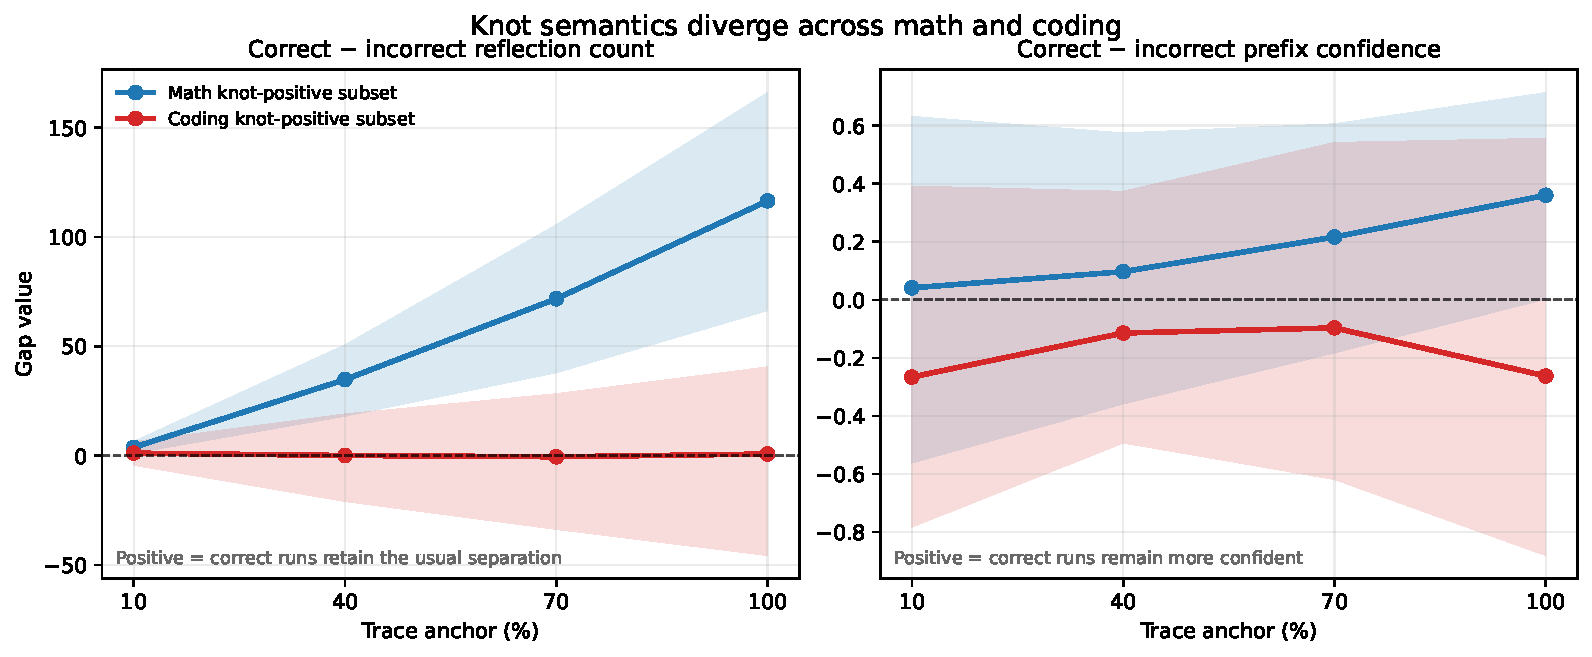
\includegraphics[width=\linewidth]{fig_knot_domain_profiles_v3.pdf}
    \caption{Mean feature gap inside the break-positive pilot subsets. The plotted quantity is correct-minus-incorrect mean value at each anchor; shaded bands show 95\% cluster-bootstrap intervals. Left: \texttt{traj\_reflection\_count}. Right: \texttt{tok\_conf\_prefix}.}
    \label{fig:knotprofiles}
\end{figure}

The label-pattern summaries point in the same direction. On the math side, \texttt{double\_definition} appears on both correct and incorrect runs, while \texttt{unresolved\_repair} is concentrated on incorrect runs. On the coding side, the dominant states are \texttt{lost\_state} and \texttt{patchy\_backtracking}. The safest interpretation is still conditional:
\begin{quote}
\textbf{The small validation study is consistent with different failure structure in math and coding: math break-like events can coexist with successful rebinding and recovery, whereas coding break-like events are more tightly tied to unstable state serialization.}
\end{quote}

This is mechanism-supporting evidence, not a finished taxonomy claim.

\section{Limitations and Conclusion}

This is an observational study, and its limits should be stated directly.

First, the probe is intentionally simple. That helps interpretability, but it is also a limitation. The paper does not claim state-of-the-art verifier accuracy, nor does it compare against hidden-state probes, stronger coding-specific verifiers, or generative verifier architectures. A small MLP sanity check reduces the risk that the cross-domain pattern is a purely linear-head artifact, but it is not a substitute for broader baseline coverage.

Second, the local-state-break study remains partly exploratory. The expanded math pilot now covers 256 selected runs, 245 parsed runs, and 490 quote-level verification decisions. The coding side now also includes a 240-run GLM-assisted audit with manual author review of sampled outputs, plus a 450-example onset-localization extension. But the timing localization succeeds in only 272 of those 450 cases, and none of these components amounts to an independent human-annotation campaign. They should therefore be read as protocol validation and mechanism-supporting evidence, not as population-level estimates of knot prevalence or a finished cross-domain taxonomy. The strongest claims in the paper do \emph{not} depend on these studies alone. They depend on the full-scale positive math/science result and the full-scale negative coding result.

Third, this workshop version deliberately focuses on domain conditioning. Regime-conditioned verifier drift under RL is important, but it is split into a separate short paper in this repository in order to keep the present manuscript on one coherent axis.

With those limits in place, the main conclusion is still clear:
\begin{quote}
\textbf{CoT self-correction is not a universal quality signal. In math/science it can support a transferable verifier; in coding the same interpretable feature family becomes weak; and the expanded coding-side audits remain more consistent with domain-specific failure structure than with one universal event.}
\end{quote}

The practical lesson is straightforward. Before deploying a CoT-based verifier, it is not enough to measure whether the feature family is predictive somewhere. One must also check whether the \emph{meaning} of those features is stable in the target domain. In coding, the added feature screen narrows this point further: the stronger signals are still weak, and they do not line up with a simple static complexity explanation.

\paragraph{Artifacts.}
Main quantitative claims are reproduced from \texttt{results/tables/} and \texttt{docs/}. The validation and comparison scripts are in \texttt{scripts/}; the current draft is in \texttt{workshop/}.

\bibliographystyle{plainnat}
\begin{thebibliography}{13}

\bibitem{wei2022cot}
Jason Wei, Xuezhi Wang, Dale Schuurmans, Maarten Bosma, Brian Ichter, Fei Xia, Ed Chi, Quoc Le, and Denny Zhou.
\newblock Chain-of-thought prompting elicits reasoning in large language models.
\newblock In \emph{NeurIPS}, 2022.

\bibitem{wang2023selfconsistency}
Xuezhi Wang, Jason Wei, Dale Schuurmans, Quoc Le, Ed Chi, Sharan Narang, Aakanksha Chowdhery, and Denny Zhou.
\newblock Self-consistency improves chain of thought reasoning in language models.
\newblock In \emph{ICLR}, 2023.

\bibitem{cobbe2021training}
Karl Cobbe, Vineet Kosaraju, Mohammad Bavarian, Mark Chen, Heewoo Jun, Lukasz Kaiser, Matthias Plappert, Jerry Tworek, Jacob Hilton, Reiichiro Nakano, et al.
\newblock Training verifiers to solve math word problems.
\newblock \emph{arXiv preprint arXiv:2110.14168}, 2021.

\bibitem{lightman2023verify}
Hunter Lightman, Vineet Kosaraju, Yura Burda, Harri Edwards, Bowen Baker, Teddy Lee, Jan Leike, John Schulman, Ilya Sutskever, and Karl Cobbe.
\newblock Let's verify step by step.
\newblock \emph{arXiv preprint arXiv:2305.20050}, 2023.

\bibitem{wang2024mathshepherd}
Peiyi Wang, Lei Li, Zhihong Shao, Ruochen Xu, Deli Chen, Ningyu Zhang, Yulin Chen, Wei Xu, and Enhong Chen.
\newblock Math-Shepherd: Verify and reinforce {LLM}s step-by-step without human annotations.
\newblock In \emph{ACL}, 2024.

\bibitem{zheng2025processbench}
Chujie Zheng, Yuxin Peng, Chenyang Wang, Shiqi Wang, and Lei Sha.
\newblock ProcessBench: Identifying process errors in mathematical reasoning.
\newblock In \emph{ACL}, 2025.

\bibitem{zhang2025genrm}
Lunjun Zhang, Yin Luo, Biwei Huang, Yixuan Wei, Zichao Zhong, and Lei Sha.
\newblock Generative verifiers: Reward modeling as next-token prediction.
\newblock In \emph{ICLR}, 2025.

\bibitem{lanham2023faithfulness}
Tamas K. Feher de Lanham, Victor Veitch, Jasper Ho, Nora Belrose, Tamkin Alex, Marvin Zhang, Sebastian Riedel, and Ethan Perez.
\newblock Measuring faithfulness in chain-of-thought reasoning.
\newblock \emph{arXiv preprint arXiv:2307.13702}, 2023.

\bibitem{liu2024intrinsic}
Dancheng Liu, Yifei Yang, Weihao Yuan, Yilun Du, and Andrew Chi-Chih Yao.
\newblock Large language models have intrinsic self-correction ability.
\newblock In \emph{NeurIPS}, 2024.

\bibitem{madaan2023selfrefine}
Aman Madaan, Niket Tandon, Prakhar Gupta, Skyler Hallinan, Luyu Gao, Sarah Wiegreffe, Uri Alon, Nouha Dziri, Shrimai Prabhumoye, Yiming Yang, et al.
\newblock Self-Refine: Iterative refinement with self-feedback.
\newblock \emph{arXiv preprint arXiv:2303.17651}, 2023.

\bibitem{shinn2023reflexion}
Noah Shinn, Federico Cassano, Edward Berman, Ashwin Gopinath, Karthik Narasimhan, and Shunyu Yao.
\newblock Reflexion: Language agents with verbal reinforcement learning.
\newblock \emph{arXiv preprint arXiv:2303.11366}, 2023.

\bibitem{huang2024selfcorrect}
Jie Huang, Xinyun Chen, Swaroop Mishra, Huaixiu Steven Zheng, Adams Wei Yu, Xinying Song, and Denny Zhou.
\newblock Large language models cannot self-correct reasoning yet.
\newblock \emph{arXiv preprint arXiv:2310.01798}, 2023.

\end{thebibliography}

\end{document}
